
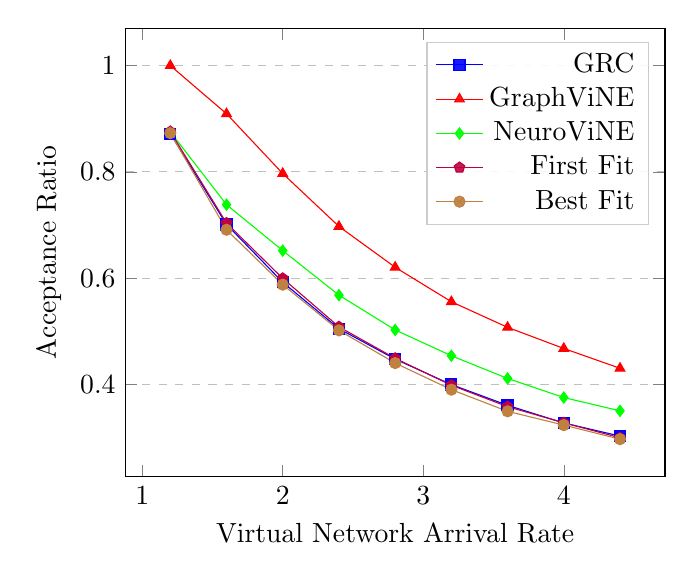
\begin{tikzpicture}
\begin{axis}[
    legend cell align={right},
    legend style={fill opacity=0.9, draw opacity=1, text opacity=1, draw=white!80!black},
    xlabel={Virtual Network Arrival Rate},
    ylabel={Acceptance Ratio},
    legend pos=north east,
    ymajorgrids=true,
    grid style=dashed,
]

\addplot[
    color=blue,
    mark=square*,
    ]
    coordinates {
(1.2,0.8720300125052105)
(1.6,0.7011566114410753)
(2.0,0.5923980995248812)
(2.4,0.5050020842017507)
(2.8,0.44783851375491246)
(3.2,0.39987494137877133)
(3.6,0.3608447964429623)
(4.0,0.3276228585719645)
(4.4,0.30297862664847663)
    };
\addlegendentry{GRC}

\addplot[
    color=red,
    mark=triangle*,
    ]
    coordinates {
(1.2,1.0)
(1.6,0.9093466708346358)
(2.0,0.7969492373093273)
(2.4,0.6973739057940809)
(2.8,0.6205787781350482)
(3.2,0.5557292480850399)
(3.6,0.507572599694317)
(4.0,0.46780042515943476)
(4.4,0.4305366075488859)
    };
\addlegendentry{GraphViNE}

\addplot[
    color=green,
    mark=diamond*,
    ]
    coordinates {
(1.2,0.8753647353063777)
(1.6,0.7383557361675523)
(2.0,0.6519129782445612)
(2.4,0.5681533972488537)
(2.8,0.502679528403001)
(3.2,0.45411911833672036)
(3.6,0.4114214255939975)
(4.0,0.37551581843191195)
(4.4,0.35050022737608)
    };
\addlegendentry{NeuroViNE}

\addplot[
    color=purple,
    mark=pentagon*,
    ]
    coordinates {
(1.2,0.8757815756565236)
(1.6,0.7036573929352923)
(2.0,0.5996499124781196)
(2.4,0.5085452271779909)
(2.8,0.4492675955698464)
(3.2,0.3986243551664843)
(3.6,0.358343754342087)
(4.0,0.3279979992497186)
(4.4,0.29979536152796726)
    };
\addlegendentry{First Fit}

\addplot[
    color=brown,
    mark=otimes*,
    ]
    coordinates {
(1.2,0.8728636932055023)
(1.6,0.6911534854642076)
(2.0,0.5878969742435609)
(2.4,0.5018757815756565)
(2.8,0.44033583422650946)
(3.2,0.3903392215100828)
(3.6,0.34959010698902315)
(4.0,0.3236213580092535)
(4.4,0.29718053660754884)
    };
\addlegendentry{Best Fit}





\end{axis}
\end{tikzpicture}

